\chapter{評価}
\label{evaluation}
本章では,第\ref{proposal}章及び第\ref{implementation}章で設計・実装に関して述べた本提案手法に関して,第\ref{issue:cplane}節で指摘したコントロールプレーンの再利用性の課題に対して有効性を示しつつ,データプレーンが高速化できていることを評価する.
\section{評価要件}
% \label{evaluation:requirements}
% SIIT-DCにおけるダイナミックEAMT機構では,第\ref{consideration:points}節で述べた事項の充足が求められる.
% それらを定量的に評価するための指標・尺度について記述する.


% \subsection{BR間のEAMTの一貫性}
% \label{evaluation:requirements:consistency}

% SIIT-DCネットワークにおける各BRは一貫性のあるEAMTを保持する必要がある.
% 本評価実験では後に述べるテストケースにおいて,以下の2点を検証することで各BRのEAMTが一貫性を有すると定義する.
% \begin{itemize}
%     \item \textbf{EAM数の収束} \\
%     EAMの更新が行われる事象が発生した場合に,一定の収束時間が経過した後に各BRのEAMTのレコード数が変化することなく,一意に収束すること.
%     \item \textbf{EAMTのレコードの内容} \\
%     EAM数が収束した際に各BRの有するEAMTの内容に差異が無いこと.
% \end{itemize}

% \subsection{変更追従性}
% \label{evaluation:requirements:change}
% 前に述べたように,従来のSIIT-DCの構成では,IPv4サービスが追加・削除・変更された場合やBRの追加配備を行った場合に,各BRのEAMTの内容を適宜変更する必要があった.

% 本研究ではEAMT変更が必要な事象が発生した場合に,運用者が特別なオペレーションを行うことなくサービス提供を想定通りに開始・継続・中断される状況を,EAMTが変更に追従している状態であると定義する.

% 本評価実験では下記の様なEAMT変更が必要な事象のうち,IPv4サービの追加・削除について検証する.

% \begin{itemize}
%     \item \textbf{IPv4サービスの追加・削除} \\
%     ネットワーク内のIPv6サービスにおいて,IPv4サービスアドレスを付与することでIPv4/IPv6の両プロトコルによるサービス提供を開始する場合.もしくは,そのサーバが行っているIPv4サービス提供を中断する場合.
%     \item \textbf{IPv4サービス提供サーバの変更} \\
%     SIIT-DCにおいて提供中のIPv4サービスに関して,他のIPv6アドレスを持つサーバによるサービス提供を改めて開始する場合.
%     \item \textbf{BRの追加・撤去} \\ 
%     対外接続点に新しいBRを追加もしくは稼働中のBRを撤去しながらIPv4サービスを継続して行う場合.
% \end{itemize}


% \subsection{スケーラビリティ}
% \label{evaluation:requirements:scalability}
% ダイナミックEAMTを実現する機構は対外接続点やIPv4提供サービスの増加に柔軟に対応可能であることが望ましい.

% 本評価実験では各ノードのスケールにおいては下記を想定した評価試験用ネットワークを実装する.
% IPv4提供サービスの総数が増加した場合においても,本提案手法が動作が可能であることを評価する.

% \begin{itemize}
%     \item BR: 30ホスト 
%     \item ルートリフレクタ: 2ホスト 
%     \item IPv4提供サーバ: 10 〜 1000ホスト
% \end{itemize}


% \section{実験環境}
% \label{evaluation:environment}

% 本評価実験で利用した実験環境について述べる.

% \subsection{ネットワークトポロジ}
% \begin{figure}[H]
%     \begin{center}
%     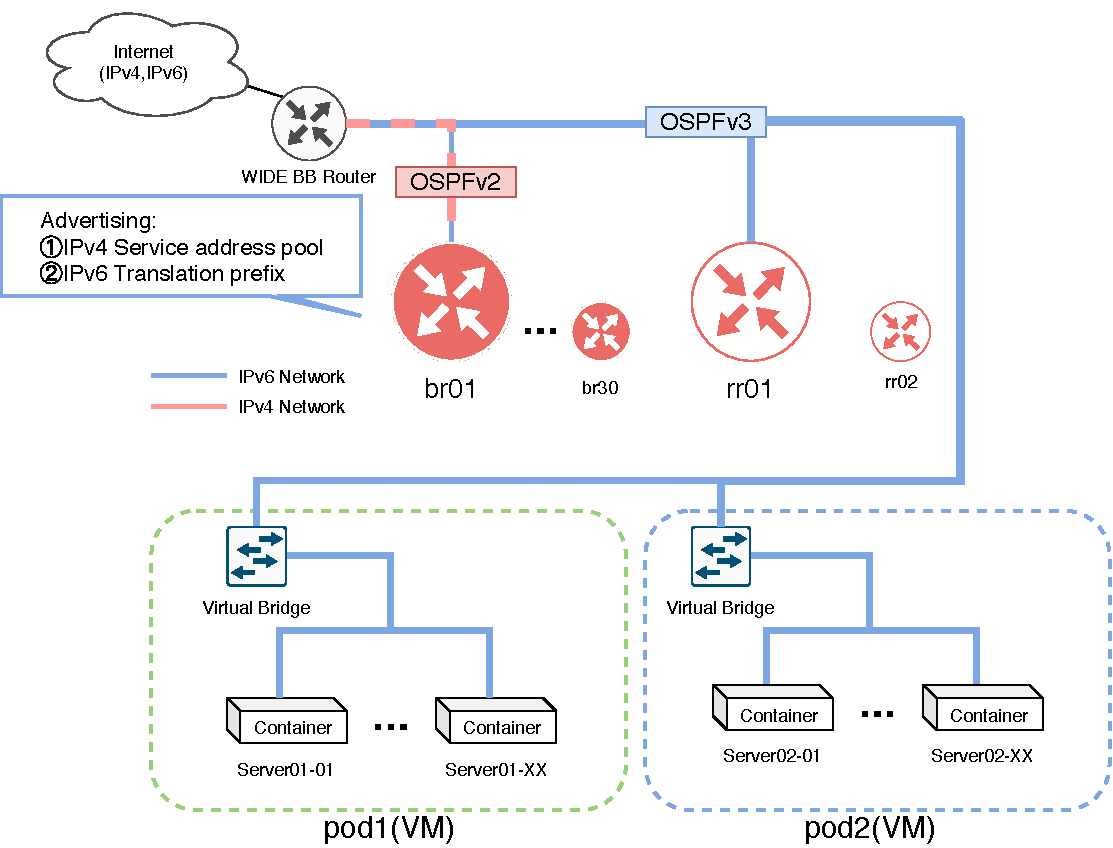
\includegraphics[width=15cm,pagebox=cropbox,clip]{img/evaluation_experiment_no_injector.pdf}
%     \end{center}
%     \caption{評価実験におけるネットワークと各ホスト}
%     \label{fig:evaluation_experiment}
% \end{figure}

% 本評価実験を行うために,WIDEプロジェクト\footnote{\url{https://www.wide.ad.jp/}}藤沢NOC内に実験用ネットワークを構築した.図\ref{fig:evaluation_experiment}に本評価実験用ネットワークの概略を示す.
% 本ネットワークでは第\ref{issue:siit-dc-merit:scalability}項で述べたECMPエニーキャストによるBRの水平スケールを可能にするネットワークトポロジを採用している.


% 本ネットワークでは,BR群(br01 $\cdots$ br30)のみ,WIDEネットワークを介してIPv4インターネットに接続している.WIDEプロジェクト内のルータに対して,IPv4サービス提供サーバ群(Server01-01  $\cdots$ Server02-60)が利用するIPv4サービスアドレス群を,OSPFv2\cite{RFC2328}を利用したECMPエニーキャストにて広告する.これにより,インターネット上のIPv4クライアントからのIPv4パケットはいずれかのBRを経由し,ダイナミックEAMTを参照したSIITによるネットワークプロトコル変換が各BRにて行われたのち,IPv6パケットとして各IPv4サービス提供サーバに転送される.

% 各ホストは共通のIPv6ネットワーク上に所属し,WIDEネットワークを介してインターネット疎通性を持つ.このIPv6ネットワークでは,各BRからIPv4サービス提供サーバ向けに,OSPFv3\cite{RFC5340}を利用したECMPエニーキャストによる変換プレフィックス向けの経路広告が行われている.IPv4サービス提供サーバからの変換プレフィックス宛のパケットは,いずれかのBRを経由してSIITによるネットワークプロトコル変換がなされたあと,インターネット上のIPv4提供クライアントに向けて返送される.

% 各ホスト間のダイナミックEAMTに用いるBGPメッセージングは,各ホストが共通して属するIPv6ネットワークを介して行われる.BR群及びIPv4サービス提供サーバ群はルートリフレクタ群(rr01 $\cdots$ rr02)に対して,IPv6によるIBGPコネクションを確立する.本ネットワークではルートリフレクタ間のBGPメッセージングは行わない一層のルートリフレクタ構成を採用する.各IPv4サービス提供サーバからの経路情報は,ネットワーク内で一意のクラスタIDを付与した上でBR群に広告される.

% なお,本実験環境ではBGPコネクションを維持するための各種パラメータを表\ref{table:eval_bgp_timer}の様に指定する.

% 各ホストは各BRはNTP(Network Time Protocol)\cite{RFC5905}を利用した時刻同期を行う.同一ネットワーク上のNTPサーバを参照元とし,十分な精度で同期を行っていると仮定する.


% \begin{table}[]
%     \label{table:eval_bgp_timer}
%     \caption{BGPコネクションで利用したパラメータ}
%     \centering
%     \resizebox{\textwidth}{!}{%
%     \begin{tabular}{lcl}
%     \hline
%     \multicolumn{1}{c}{要素} & 値 & \multicolumn{1}{c}{説明} \\ \hline
%     Keep Alive Interval & 3秒 (標準:60秒) & KEEPALIVEメッセージの送信間隔 \\
%     Hold Time & 9秒 (標準:180秒) & この値以上KEEPALIVEの到達を確認出来なかった場合,当該ピアから受信した経路を破棄する. \\
%     ConnectTimer & 5秒 (標準:120秒) & BGPコネクションの再試行を行う間隔. \\ \hline
%     \end{tabular}%
%     }
% \end{table}

% \subsection{実装}
% 本項では各ホストの実行環境について記述する.
% 各ホストが利用している,BGPデーモン・SIIT機構・EAMT制御機構の各コンポーネントは,第\ref{implementation:poc:components}項で述べたPoCと同一の物を利用している.


% \subsubsection{BR}
% 本評価ネットワークにおけるBR群は,同一物理サーバ上で仮想マシンとして稼働する.
% 表\ref{table:eval_env_BR}に物理サーバと仮想マシンの実行環境を詳細に示す.

% また,各BR上で現在保有しているEAMT数・BGP経路数を計測するための監視プロセスを0.2秒毎に実行し,各種評価要件の検証に利用する.

% \begin{table}[h]
%     \label{table:eval_env_BR}
%     \caption{評価実験用BR群の実行環境}
%     \resizebox{\textwidth}{!}{%
%     \begin{tabular}{|cccc}
%     \hline
%     \multicolumn{4}{|c|}{\cellcolor[HTML]{EFEFEF}\textbf{計算環境}} \\ \hline
%     \multicolumn{1}{|c|}{機種} & \multicolumn{1}{c|}{CPU} & \multicolumn{1}{c|}{RAM} & \multicolumn{1}{c|}{NIC} \\ \hline
%     Intel S2600WTT & 2CPU: Intel Xeon E5-2699 v3 2.30GHz & 64GB & \multicolumn{1}{c|}{Intel 82599EB 10-Gigabit SFI/SFP+} \\ \hline
%     \multicolumn{4}{|c|}{\cellcolor[HTML]{EFEFEF}\textbf{ハイパーバイザ環境}} \\ \hline
%     \multicolumn{1}{|c|}{OS} & \multicolumn{1}{c|}{バージョン} & \multicolumn{1}{c|}{vCPU} & \multicolumn{1}{c|}{備考} \\ \hline
%     VMware ESXi & 6.7.0 & 72 & \multicolumn{1}{l|}{build: 5160138} \\ \hline
%     \multicolumn{4}{|c|}{\cellcolor[HTML]{EFEFEF}\textbf{仮想マシン}} \\ \hline
%     \multicolumn{1}{|c|}{OS} & \multicolumn{1}{c|}{カーネル} & \multicolumn{1}{c|}{リソース} & \multicolumn{1}{c|}{利用コンポーネント} \\ \hline
%     Ubuntu 18.04.3 LTS & 4.15.0-72-generic & vCPU: 2 RAM:2GB & \multicolumn{1}{l|}{BGPデーモン,EAMT制御機構,SIIT機構} \\ \hline
%     \end{tabular}%
%     }
% \end{table}





% \subsubsection{ルートリフレクタ}
% 本評価ネットワークにおけるルートリフレクタ群は,同一物理サーバ上仮想マシンとして稼働する.
% 表\ref{table:eval_env_RR}に物理サーバと仮想マシンの実行環境を詳細に示す.

% 本ルートリフレクタではBGPデーモンにて,ルートリフレクタ機能に加えてダイナミックネイバー機能を有効化する.通常BGPコネクションを確立するためには,BGPピア間で互いのピアリングアドレスを明示的に設定する必要があるが,本機能を利用することで動的に多数のBGPスピーカとのピアリングが可能になる\cite{GoBGP_dynamic}.同様の機構は他のBGP実装やネットワーク機器にも搭載されている\cite{Cisco_dynamic}.


% \begin{table}[]
%     \label{table:eval_env_RR}
%     \caption{評価実験用RR群の実行環境}
%     \resizebox{\textwidth}{!}{%
%     \begin{tabular}{|cccc}
%     \hline
%     \multicolumn{4}{|c|}{\cellcolor[HTML]{EFEFEF}\textbf{計算環境}} \\ \hline
%     \multicolumn{1}{|c|}{機種} & \multicolumn{1}{c|}{CPU} & \multicolumn{1}{c|}{RAM} & \multicolumn{1}{c|}{NIC} \\ \hline
%     Dell PowerEdge R410 & 2CPU: Intel Xeon E5530 @ 2.40GHz & 16GB & \multicolumn{1}{c|}{HP NC522SFP Dual Port 10GbE Server Adapter} \\ \hline
%     \multicolumn{4}{|c|}{\cellcolor[HTML]{EFEFEF}\textbf{ハイパーバイザ環境}} \\ \hline
%     \multicolumn{1}{|c|}{OS} & \multicolumn{1}{c|}{バージョン} & \multicolumn{1}{c|}{vCPU} & \multicolumn{1}{c|}{備考} \\ \hline
%     VMware ESXi & 6.5.0 & 16 & \multicolumn{1}{l|}{build: 15256549.} \\ \hline
%     \multicolumn{4}{|c|}{\cellcolor[HTML]{EFEFEF}\textbf{仮想マシン}} \\ \hline
%     \multicolumn{1}{|c|}{OS} & \multicolumn{1}{c|}{カーネル} & \multicolumn{1}{c|}{リソース} & \multicolumn{1}{c|}{利用コンポーネント} \\ \hline
%     Ubuntu 18.04.3 LTS & 4.15.0-72-generic & vCPU: 4 RAM:4GB & \multicolumn{1}{l|}{BGPデーモン} \\ \hline
%     \end{tabular}%
%     }
% \end{table}

% \subsubsection{IPv4サービス提供サーバ}
% 本実験環境において,IPv4サービス提供サーバ群はコンテナ型仮想化\cite{soltesz2007container}を利用し,二つのホスト仮想マシン上で実行される.
% 図\ref{table:eval_env_server}に物理サーバとホスト仮想マシン及びコンテナの実行環境を詳細に示す.


% \begin{table}[h]
%     \label{table:eval_env_server}
%     \caption{評価実験用IPv4サービス提供サーバ群の実行環境}
%     \resizebox{\textwidth}{!}{%
%     \begin{tabular}{|cccc}
%     \hline
%     \multicolumn{4}{|c|}{\cellcolor[HTML]{EFEFEF}\textbf{計算環境}} \\ \hline
%     \multicolumn{1}{|c|}{機種} & \multicolumn{1}{c|}{CPU} & \multicolumn{1}{c|}{RAM} & \multicolumn{1}{c|}{NIC} \\ \hline
%     Dell PowerEdge R410 & 2CPU: Intel Xeon E5530 @ 2.40GHz & 48GB & \multicolumn{1}{c|}{HP NC522SFP Dual Port 10GbE Server Adapter} \\
%     \multicolumn{1}{|l}{Dell PowerEdge R410} & \multicolumn{1}{l}{2CPU: Intel Xeon E5530 @ 2.40GHz} & 48GB & \multicolumn{1}{l|}{HP NC522SFP Dual Port 10GbE Server Adapter} \\ \hline
%     \multicolumn{4}{|c|}{\cellcolor[HTML]{EFEFEF}\textbf{ハイパーバイザ環境}} \\ \hline
%     \multicolumn{1}{|c|}{OS} & \multicolumn{1}{c|}{バージョン} & \multicolumn{1}{c|}{vCPU} & \multicolumn{1}{c|}{備考} \\ \hline
%     VMware ESXi & 6.5.0 & 16 & \multicolumn{1}{l|}{build: 15256549. Pod1,Pod2で共通} \\ \hline
%     \multicolumn{4}{|c|}{\cellcolor[HTML]{EFEFEF}\textbf{ホスト仮想マシン}} \\ \hline
%     \multicolumn{1}{|c|}{OS} & \multicolumn{1}{c|}{カーネル} & \multicolumn{1}{c|}{リソース} & \multicolumn{1}{c|}{備考} \\ \hline
%     Ubuntu 18.04.3 LTS & 4.15.0-72-generic & vCPU: 4 RAM:4GB & \multicolumn{1}{l|}{Pod1, Pod2で共通} \\ \hline
%     \multicolumn{4}{|c|}{\cellcolor[HTML]{EFEFEF}\textbf{コンテナ}} \\ \hline
%     \multicolumn{1}{|c|}{OS} & \multicolumn{1}{c|}{コンテナエンジン} & \multicolumn{1}{c|}{コンテナイメージ} & \multicolumn{1}{c|}{利用コンポーネント} \\ \hline
%     Alpine Linux 3.11 & Dockerversion 19.03.5 & 自作 & \multicolumn{1}{l|}{GoBGPデーモン} \\ \hline
%     \end{tabular}%
%     }
% \end{table}


% \section{評価実験1: EAMTの収束・一貫性の検証}
% \label{evaluation:eval1}

% 本節では\ref{evaluation:requirements}項で述べた三つの要件のうち,「BR間のEAMTの一貫性」及び「スケーラビリティ」の検証を目的とした評価実験を行い,その詳細と結果について述べる.

% \subsection{シナリオ}
% 基本的なSIIT-DCネットワークの構築を想定し,IPv4提供サービスサーバ群を起動した後に,BR間のEAMTの一貫性が正しく維持されるかを検証する.

% \subsubsection{手順}
% 以下のような手順を1単位として,IPv4サービス提供サーバ数$x$につき1回試行する.
% \begin{enumerate}
%     \item \textbf{ルートリフレクタの起動} \\
%     ルートリフレクタ群を起動し,BGPデーモンの立ち上げを確認する.
%     \item \textbf{BRの起動} \\
%     BR群を起動し,BGPデーモン・EAMT制御機構の立ち上げを確認する.
%     \item \textbf{IPv4サービス提供サーバの起動} \\
%     IPv4サービス提供サーバを$x$ホスト起動し,それぞれのサーバにおいてBGPデーモンの立ち上げ及びEAM情報のLoc-RIBへの反映を確認する.この時利用するIPv4サービスアドレスは事前に作成した正答となるEAMTを参照する.実験環境の都合上,サーバの起動は同期的に行う.
%     \item \textbf{計測} \\
%     全てのサーバが起動の起動を確認し,サーバの起動から30秒後の各BRのEAMTの状態を収集する.EAMTの内容を,事前に作成した正答となるEAMTと比較する.
% \end{enumerate}

% \subsection{説明変数・目的変数}
% 本実験環境におけるBRの数を$B$,事前に作成したEAMTに正答したBRの数$B_s$とし,正答率$R$を目的変数とする.
% 目的変数$R$は以下の様な式\ref{eq:eval1}で表す事ができる.またIPv4サービス提供サーバの数を$x$とし,本評価実験の説明変数とする.

% \begin{equation}
%     R = \frac{B_s}{B}
%     \label{eq:eval1}
% \end{equation}


% \subsection{条件}
% 各ホストの情報を表\ref{table:eval1_condition}に示す.ここに記載の無いはその他の条件は\ref{evaluation:environment}項に準ずる.

% \begin{table}[]
%     \label{table:eval1_condition}
%     \caption{評価実験1での各ホストの情報}
%     \resizebox{\textwidth}{!}{%
%     \begin{tabular}{lcl}
%     \hline
%     \multicolumn{1}{c}{要素} & ホスト数 & ホスト名 \\ \hline
%     BR & 30 & br01〜br30 \\
%     ルートリフレクタ & 2 & rr01〜rr02 \\
%     IPv4サービス提供サーバ & 10,100,200,400,500,600,700,800,900,1000& server01-01 〜 server01-500, server02-01 〜 server02-500 \\ \hline
%     \end{tabular}%
%     }
% \end{table}


% \subsection{結果と考察}
% \label{evaluation:eval1:result}
% 本評価実験の結果を表\ref{table:eval1_result}に示す.

% IPv4提供サービスサーバ数$x$が600までの場合に,全てのBR間で保有するEAMTが収束し,一貫性を維持していることが読み取れる.
% 一方で$x>=700$の場合には全てのBRのEAMTが正答に一致しておらず,且つ収束しないことがわかった.


% \begin{table}[]
%     \label{table:eval1_result}
%     \caption{評価実験1での各ホストの情報}
%     \centering
%     \resizebox{\textwidth}{!}{%
%     \begin{tabular}{lcl}
%     \hline
%     \multicolumn{1}{c}{$x$: IPv4サービス提供サーバの数} & $R$: 正答にEAMTが一致したBR数の割合 & EAMTの収束可否 \\ \hline
%     10 & 100 \% & 収束 \\
%     100 & 100 \% & 収束 \\
%     200 & 100 \% & 収束 \\
%     300 & 100 \% & 収束 \\
%     400 & 100 \% & 収束 \\
%     500 & 100 \% & 収束 \\
%     600 & 100 \% & 収束 \\
%     700 & 0 \% & 収束せず \\
%     800 & 0 \% & 収束せず \\
%     900 & 0 \% & 収束せず \\
%     1000 & 0 \% & 収束せず \\ \hline
%     \end{tabular}%
%     }
% \end{table}


% \begin{minipage}{\textwidth}
%     \begin{lstlisting}[caption=EAMTが収束しない時点のルートリフレクタのログの抜粋,label=code:experiment1_rr]
%         Jan 06 13:11:56 rr01 gobgpd[18970]: {"Code":4,"Data":null,"Key":"2001:200:0:8831:1:0:6440:243","Subcode":0,"Topic":"Peer","level":"warning","msg":"received notification","time":"2020-01-06T13:11:56+09:00"}
%         Jan 06 13:11:56 rr01 gobgpd[18970]: {"Key":"2001:200:0:8831:1:0:6440:243","Reason":"notification-received code 4(hold timer expired) subcode 0(undefined)","State":"BGP_FSM_ESTABLISHED","Topic":"Peer","level":"info","msg":"Peer Down","time
%         Jan 06 13:12:00 rr01 gobgpd[18970]: {"Key":"2001:200:0:8831:1:0:6440:1d","State":"BGP_FSM_ESTABLISHED","Topic":"Peer","level":"warning","msg":"Closed an accepted connection","time":"2020-01-06T13:12:00+09:00"}
%     \end{lstlisting}
% \end{minipage}
    
    
% 当該期間中のルートリフレクタ(rr01)のログメッセージの抜粋をコード\ref{code:experiment1_rr}に示す.BGPピア(IPv4サービス提供サーバ)より,ルートリフレクタから送信されるBGP KEEPALIVEメッセージに問題がある旨を表すBGP NOTIFICATIONメッセージを受信していることが読み取れる.$x=700$の実験期間中,常にこのようなログメッセージが高頻度で観測されていた.本問題はルートリフレクタが一定以上のBGPピアを収容する場合,正常にKEEPALIVEメッセージを送信出来ず,全体のBGPコネクションの維持に問題が生じていることに起因することがわかる.


% 本評価実験を通して,本提案手法がEAMTの一貫性の維持に効果的に作用することがわかった.
% しかしながら本評価環境においては,ルートリフレクタが収容できるBGPコネクションに限りがあり,ルートリフレクタが保有するBGPコネクションの数が一定の値を超えた場合に,全てのBRのEAMTが維持できなくなる課題が明らかになった.




% \section{評価実験2: 構成変更追従性の検証}
% \label{evaluation:eval2}
% 本節では\ref{evaluation:requirements}項で述べた三つの要件のうち,「変更追従性」「スケーラビリティ」の検証を目的とした評価実験を行い,その詳細と結果について記述する.



% \subsection{シナリオ}
% IDCネットワークにおいてIPv4サービス構成が変更になったことを想定し,変更が発生した時点から各BRのEAMTが一貫性を維持するまでの経過時間を計測する.

% \subsubsection{構成変更の定義}
% \label{evaluation:eval2:scenario:definication}
% 本評価実験では以下の二つの事例を「IPv4サービス提供サーバの構成変更」と定義する.

% \begin{enumerate}
%     \item \textbf{IPv4サービス提供サーバの追加} \\
%     IPv4サービス提供サーバ1台を新規に起動し,BGPデーモンの立ち上げ及び当該サーバがIPv4サービスを行うために必要なEAMの情報を,当該サーバのLoc-RIBに反映する. 
%     \item \textbf{IPv4サービス提供サーバの削除} \\
%     任意のIPv4サービス提供サーバ宛のパケットを,ホスト仮想マシン上でフィルターし,当該サーバがルートリフレクタと疎通不能な状態を再現する.
% \end{enumerate}


% \subsubsection{手順}
% 以下のような手順を1単位として,初期状態のIPv4サービス提供サーバ数$x$につき各30回試行する.
% \begin{enumerate}
%     \item \textbf{初期状態の準備} \\
%     \ref{evaluation:eval1}節で述べた手順を完了したIPv4サービス提供サーバ$x$ホストが,各BRを介したIPv4サービスが提供可能になった状態を初期状態とする.
%     \item \textbf{IPv4サービス提供サーバの構成変更} \\
%     \ref{evaluation:eval2:scenario:definication}項で述べた二つの事例のうち,一つを実行する.
%     \item \textbf{計測} \\
%     IPv4サービス提供サーバの構成変更から,各BRのEAMTが収束\footnote{ここでは\ref{evaluation:requirements:consistency}項で述べたEAMTが一貫性を維持した状態とする.}するまでに経過した時間を計測する.
% \end{enumerate}

% \subsection{説明変数・目的変数}
% \label{evaluation:eval2:scenario:vars}

% 第\ref{implementation:poc:sequence}項で述べた本提案手法のメッセージングのシーケンスから,IPv4サービス提供サーバの追加・削除に関わるものを抜粋する.

% \subsubsection{IPv4サービス提供サーバの追加後のプロセス}
% BRのEAMTがIPv4サービス提供サーバの追加に追従するまでに必要な各コンポーネントの動作は,以下の5つの段階に分類することが出来る.

% \begin{enumerate}
%     \item IPv4サービス提供サーバが自身のLoc-RIBにEAMを反映
%     \item IPv4サービス提供サーバとルートリフレクタ間のBGPコネクションの確立
%     \item IPv4サービス提供からBGP UPDATEメッセージがルートリフレクタに伝達
%     \item ルートリフレクタが各BR及びにUPDATEメッセージを送信
%     \item 各BRが自身のLoc-RIBを変更しEAMTを更新
% \end{enumerate}

% 目的変数$T_a$は以下の様な式\ref{eq:eval2_1}で表す事ができる.本実験環境におけるBRの数を$B$,IPv4サービス提供サーバ1台がコネクション確立に掛かる時間を$t_c$,IPv4サービス提供サーバ1台がBGP UPDATEメッセージをルートリフレクタに伝達するまでに掛かる時間を$t_u$,ルートリフレクタが1台のBRにUPDATEメッセージを送信するのに掛かる時間を$t_b$,1台のBRがLoc-RIBを変更しEAMTを更新するまでに掛かる時間を$t_e$,IPv4サービス提供サーバの数を$x$とし,$x$を本評価実験の説明変数とする.なお,各BRは同一の時間$t_e$で並行してEAMTを更新するものとする.

% \begin{equation}
%     T_a = t_c + t_u + B \cdot x \cdot t_b + t_e
%     \label{eq:eval2_1}
% \end{equation}

% \subsubsection{IPv4サービス提供サーバの削除後のプロセス}
% また,IPv4サービス提供サーバの削除を行う場合,IPv4サービス提供サーバの削除からEAMTの収束までの各動作は以下のように分類される.

% \begin{enumerate}
%     \item ルートリフレクタがBGP KEEPALIVEメッセージの不到達を検知
%     \item ルートリフレクタが各BR及びにUPDATEメッセージを送信
%     \item 各BRが自身のLoc-RIBを変更しEAMTを更新
% \end{enumerate}

% 目的変数$T_b$は以下の様な式\ref{eq:eval2_2}で表す事ができる.なお,各BRは同一の時間$t_e$で並行してEAMTを更新するものとする.なお,
% ルートリフレクタがBGP KEEPALIVEメッセージの不到達を検知を検知するまでの時間を$t_d$,本実験環境におけるBRの数を$B$,IPv4サービス提供サーバの数を$x$とし,$x$を本評価実験の説明変数とする.

% \begin{equation}
%     T_b = t_d + B \cdot (x-1) \cdot t_b  + t_e
%     \label{eq:eval2_2}
% \end{equation}



% \subsection{条件}
% 各ホストの情報を表\ref{table:eval1_condition}に示す.記載の無いその他の条件は\ref{evaluation:environment}項に準ずる.
% 初期状態のIPv4サービス提供サーバの数$x$に関しては,\ref{evaluation:eval1:result}項で得られた結果から妥当な数量を決定した.

% \begin{table}[h]
%     \label{table:eval2_condition}
%     \caption{評価実験2での各ホストの情報}
%     \resizebox{\textwidth}{!}{%
%     \begin{tabular}{lcl}
%     \hline
%     \multicolumn{1}{c}{要素} & ホスト数 & ホスト名 \\ \hline
%     BR & 30 & br01〜br30 \\
%     ルートリフレクタ & 2 & rr01〜rr02 \\
%     初期状態のIPv4サービス提供サーバ & 50,100,150,200,250,350,400,450,500,550,600& server01-01 〜 server01-300, server02-01 〜 server02-300 \\ 
%     追加するIPv4サービス提供サーバ & 1 & extra01-01  \\ \hline
%     \end{tabular}%
%     }
% \end{table}

% \subsection{結果と考察}
% \label{evaluation:eval2:result}
% \begin{figure}[h]
%     \begin{center}
%     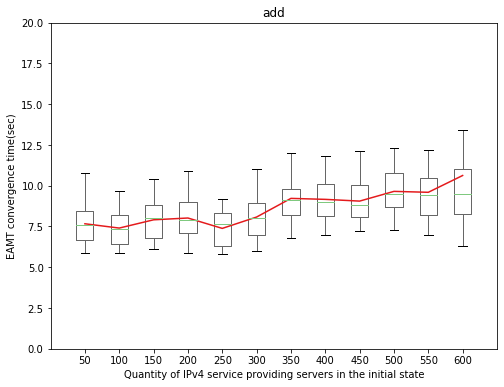
\includegraphics[width=11cm,pagebox=cropbox,clip]{img/eval2_result_add.png}
%     \end{center}
%     \caption{評価実験2:IPv4サービス提供サーバの追加を行った際のEAMT収束時間の比較}
%     \label{fig:eval2_result_add}
% \end{figure}

% \begin{figure}[h]
%     \begin{center}
%     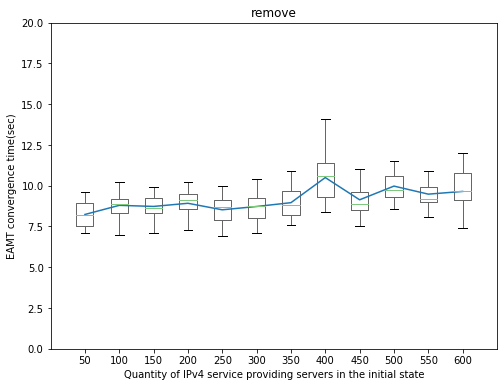
\includegraphics[width=11cm,pagebox=cropbox,clip]{img/eval2_result_remove.png}
%     \end{center}
%     \caption{評価実験2:IPv4サービス提供サーバの削除を行った際のEAMT収束時間の比較}
%     \label{fig:eval2_result_remove}
% \end{figure}

% 本評価実験の結果のうち,「IPv4サービス提供サーバの追加」を図\ref{fig:eval2_result_add}に,「IPv4サービス提供サーバの削除」を図\ref{fig:eval2_result_add}に示す.これらの図では,各説明変数$x$での試行の分布と,それぞれの平均の推移を表している.

% はじめに本評価実験の概況について考察する.いずれのケース及び説明変数$x$に於いても,各BRのEAMTが平均して概ね10秒程度で収束していることがわかる.これらの結果から,本実験環境におけるIPv4サービス提供サーバ数$x$の範囲内では,サーバ数の多寡に関わらず,変更追従機構が効果的に作用していることが評価できる.


% 次に,各ケースにおける経過時間($T_a$,$T_b$)の推移について述べる.
% IPv4サービス提供サーバの削除を行ったケースでは,初期状態のIPv4サービス提供サーバ数$x$に関わらずEAMTの収束に掛かる時間$T_b$はほぼ横ばいに推移している.一方で,サーバの追加を行ったケースでは,$x$が大きくなるに従って,EAMTの収束に掛かる時間$T_a$がなだらかに増加傾向にあることが読み取れる.

% この事象は,ルートリフレクタが保持するコネクション数が影響しているとが考えられる.IPv4サービス提供サーバ1台がコネクション確立に掛かる時間$t_c$及び,IPv4サービス提供サーバ1台がBGP UPDATEメッセージをルートリフレクタに伝達するまでに掛かる時間$t_u$が,ルートリフレクタが保有しているBGPコネクションに連動して,増加していると思われる.


% 本評価実験を通して,本提案手法の変更追従性をより機敏に機能させるためには,ルートリフレクタのコネクション数を極力抑えた設計が必要になることが明らかになった.



% \newpage
% \section{本章のまとめ}
% \label{evaluation:consideration}
% 本評価実験1の結果(\ref{evaluation:eval1:result})を通して本提案手法が各BRの一貫性の維持に有効であることを,本評価実験2の結果(\ref{evaluation:eval2:result})を通して本提案手法が変更追従性を十分に有していることをそれぞれ証明することが出来た.

% しかしながらIPv4サービス提供サーバ数$x$が一定の値より大きい場合において,ルートリフレクタが多くのBGPコネクションを保持出来ないことが明らかになっている.
% 本問題に関しては以下のような取り組みが有効であると考えられる.

% \begin{itemize}
%     \item BGPパラメータの変更 \\
%     本評価実験では,BGP KEEPALIVEメッセージージに利用する各種パラメータに関して,\ref{table:eval_bgp_timer}で指定したような値を採用している.KeepAlive送信間隔をより大きくすることで,より多くのコネクションを収容可能になることが想定される.
%     \item ルートリフレクタトポロジの見直しによる負荷軽減 \\
%     本実験環境ではルートリフレクタ2ホスト(rr01,rr02)と全てのサーバ間でBGPコネクションを確立する一層のルートリフレクタトポロジを採用しているが,第\label{proposal:network_rr}項で述べたような,1台あたりのルートリフレクタの負荷を軽減できるトポロジを取り入れることで,より多くのIPv4サービス提供サーバを本提案手法で扱うことが出来ると考えられる.
% \end{itemize}

% 両取り組みのうち,「ルートリフレクタトポロジの見直しによる負荷軽減」に関して,第\ref{conclusion:tree}節にて解決策となるBGPコネクショントポロジのデザインについて述べる.


%%% Local Variables:
%%% mode: japanese-latex
%%% TeX-master: "../thesis"
%%% End:
